\documentclass[9pt,twocolumn,twoside]{gsajnl_modified}
% Use the documentclass option 'lineno' to view line numbers

\usepackage[htt]{hyphenat}  % https://tex.stackexchange.com/a/543
\usepackage[export]{adjustbox}
\usepackage{xurl}
\usepackage{stfloats}
\usepackage[leftcaption]{sidecap}
\sidecaptionvpos{figure}{t}

\renewcommand{\topfraction}{0.9}	% max fraction of floats at top
    \renewcommand{\bottomfraction}{0.8}	% max fraction of floats at bottom
    %   Parameters for TEXT pages (not float pages):
    \setcounter{topnumber}{2}
    \setcounter{bottomnumber}{2}
    \setcounter{totalnumber}{4}     % 2 may work better
    \setcounter{dbltopnumber}{2}    % for 2-column pages
    \renewcommand{\dbltopfraction}{0.9}	% fit big float above 2-col. text
    \renewcommand{\textfraction}{0.07}	% allow minimal text w. figs
    %   Parameters for FLOAT pages (not text pages):
    \renewcommand{\floatpagefraction}{0.7}	% require fuller float pages
	% N.B.: floatpagefraction MUST be less than topfraction !!
    \renewcommand{\dblfloatpagefraction}{0.7}	% require fuller float pages

\newcommand\jdbcomment[1]{\textcolor{red}{[#1]}}
\newcommand\rancomment[1]{\textcolor{blue}{[#1]}}

\title{Fitness effects of mutations to SARS-CoV-2 proteins}

\author[*]{\Large Jesse D. Bloom$^{1,2,3^*}$ and Richard A. Neher$^{4,5}$}

\affil[1]{Basic Sciences and Computational Biology, Fred Hutchinson Cancer Center

}
\affil[2]{Department of Genome Sciences, University of Washington

}
\affil[3]{Howard Hughes Medical Institute

}
\affil[4]{Biozentrum, University of Basel

}
\affil[5]{Swiss Institute of Bioinformatics

}

\keywords{}

\runningtitle{} % For use in the footer
\runningauthor{}

\begin{abstract}
Knowledge of the fitness effects of mutations to SARS-CoV-2 can inform assessment of new variants, design of therapeutics resistant to escape, and basic understanding of the function of viral proteins.
However, experimentally determining the effects of mutations is challenging: we lack tractable lab assays for many SARS-CoV-2 proteins, and comprehensive deep mutational scanning has been applied to only two of the virus's proteins.
Here we develop an approach that leverages millions of publicly available SARS-CoV-2 sequences to estimate the effects of mutations.
We first calculate how many times each mutation is expected to occur along the SARS-CoV-2 phylogeny in the absence of selection. 
We then compare these expected counts to the actual counts to estimate the effect of each mutation.
These estimates correlate well with deep mutational scanning measurements.
For most genes, synonymous mutations are nearly neutral, stop-codon mutations are deleterious, and amino-acid mutations have a range of effects.
However, some viral accessory proteins are under little to no selection.
To enable our estimates to be easily used, we provide interactive visualizations (\url{https://jbloomlab.github.io/SARS2-mut-fitness/}).
The framework we describe is applicable to any virus for which the number of available sequences is sufficiently large that each neutral mutation independently occurs many times.
\end{abstract}

\begin{document}

\maketitle
\thispagestyle{firststyle}
%\marginmark
\firstpagefootnote

\correspondingauthoraffiliation{}{*\href{mailto:jbloom@fredhutch.org}{jbloom@fredhutch.org} or \href{mailto:richard.neher@unibas.ch}{richard.neher@unibas.ch}}
\vspace{-33pt}% Only used for adjusting extra space in the left column of the first page

\lettrine[lines=2]{\color{color2}T}{}he rapid evolution of SARS-CoV-2 has led to the repeated emergence of viral variants with enhanced transmissibility, escape from anti-viral therapeutics, or reduced recognition by immunity~\citep{harvey2021sars,abdool2021new}.
To anticipate and mitigate this evolution, the scientific community has launched major efforts to assess the risk of new viral variants~\citep{degrace2022defining} and create therapeutics that target constrained regions of the virus where resistance is less likely to evolve~\citep{moghadasi2022,iketani2022multiple,hiscox2021shutting}.
Both efforts require determining how specific mutations affect the fitness of the virus.

Unfortunately, experimentally determining the effects of mutations remains challenging for most SARS-CoV-2 proteins.
For spike, tractable laboratory assays have identified key functional and antigenic mutations~\citep{weisblum2020escape,harvey2021sars}, and enabled deep mutational scanning measurements of how most mutations affect receptor binding, cellular infection, and antibody recognition~\citep{starr2020deep,dadonaite2022pseudovirus,greaney2021complete,cao2022imprinted}.
These experimental data are valuable for assessing new spike variants~\citep{degrace2022defining,greaney2022antibody,tzou2022coronavirus} and informing development of antibody therapeutics with greater resistance to escape~\citep{starr2021sars,rappazzo2021broad,cao2022rational}.
But most other viral proteins lack comparably tractable laboratory assays, despite clearly contributing to viral fitness~\citep{thorne2022evolution,syed2021rapid,mcgrath2022sars} and being the targets of efforts to develop anti-viral drugs~\citep{tao2021sars}.
The only non-spike SARS-CoV-2 protein with large-scale deep mutational scanning data is Mpro~\citep{flynn2022,iketani2022functional}, and those measurements were performed in yeast.

An alternative to experiments is to estimate the effects of mutations by analyzing natural viral sequences.
The amount of data available for such analyses has increased dramatically over the last few years with the full-genome sequencing of SARS-CoV-2 from millions of human infections.
So far analyses of these sequences have focused on analyzing expanding viral clades to identify mutations that mediate immune escape or increase transmissibility~\citep{obermeyer2022analysis,lee2022inferring,maher2022predicting}.
The basic idea is that mutations that repeatedly appear near the base of clades that increase in relative frequency are likely beneficial to the virus.
However, only a small minority of all possible mutations are beneficial, with most being nearly neutral or deleterious.
For purposes such as identifying functionally constrained drug targets or understanding the function of viral proteins, it is important to accurately estimate the effects of neutral or deleterious mutations as well as beneficial ones.
% \jdbcomment{Richard, I could not quite figure out how to fit in \citep{strelkowa2021clonal}, let me know if you have ideas.}

Here we develop a new approach that uses natural sequences to estimate the effects of mutations.
Our basic insight is that there are now so many SARS-CoV-2 sequences that all non-deleterious single-nucleotide mutations are expected to independently occur many times along the observed phylogenetic tree.
We therefore first calculate the number of expected occurrences of each mutation based on the neutral mutation spectrum of SARS-CoV-2 estimated from four-fold degenerate synonymous sites~\citep{bloom2022evolution}.
We then compare these expected occurrences to the actual occurrences in the SARS-CoV-2 tree to estimate the effect of each mutation.
The resulting estimates correlate well with existing deep mutational scanning data.
Most viral proteins have regions that are under strong selective constraints.
However the accessory proteins mostly show only weak selection against amino-acid and even stop-codon mutations.
Overall, our work demonstrates a new approach to determine the effects of mutations, and provides detailed maps of functional constraint across the SARS-CoV-2 proteome.

\section{Results}

\subsection{Estimating fitness from actual versus expected mutation counts}

\begin{figure*}
{\bf \Large A \hspace{0.47\linewidth} B}

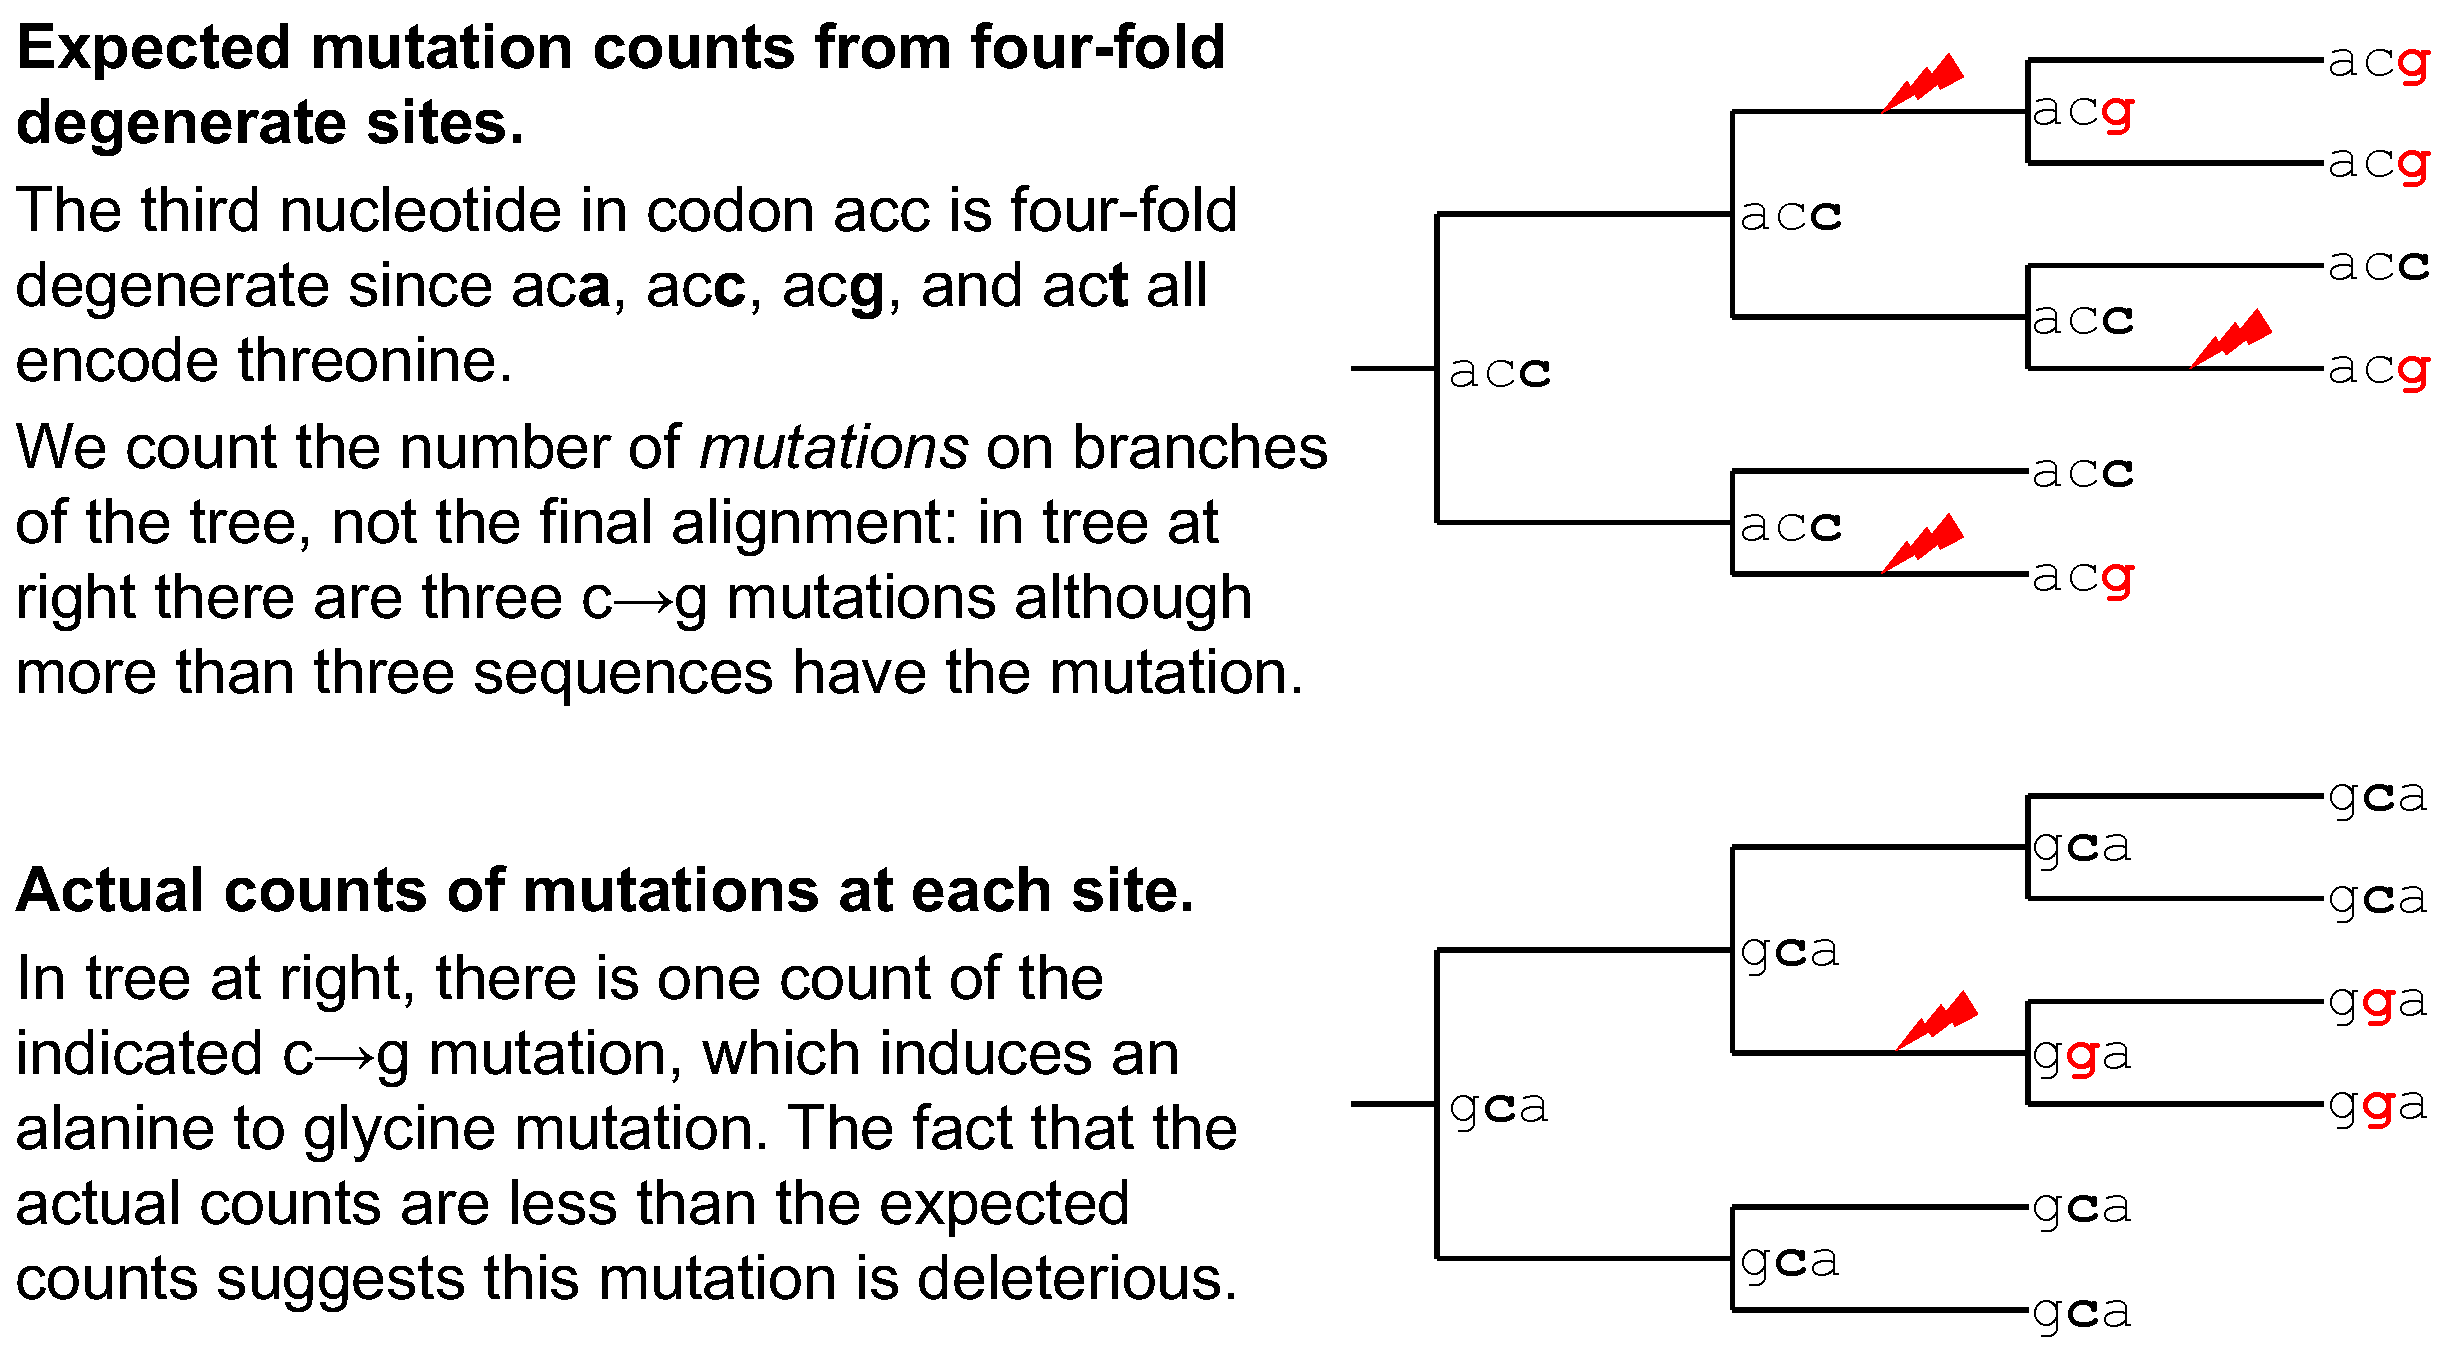
\includegraphics[width=0.48\linewidth,valign=t]{figs/schematic/schematic.pdf}
\hspace{0.02\linewidth}
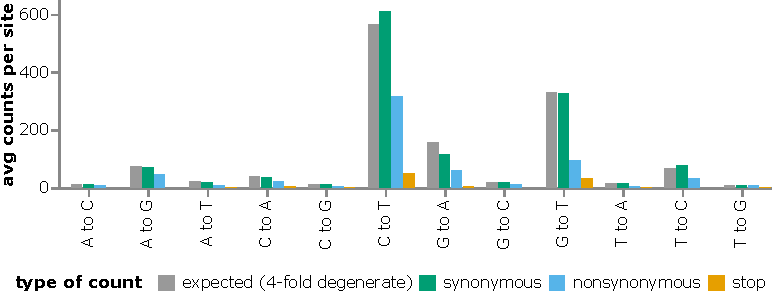
\includegraphics[width=0.5\linewidth,valign=t]{figs/avg_counts.pdf}
\caption{
Expected versus actual counts of mutations.
{\bf (A)}
The number of expected counts of each type of nucleotide mutation is computed from four-fold degenerate sites, and then compared the actual counts of each mutation.
{\bf (B)}
Expected versus actual counts for each nucleotide mutation type averaged across all sites where the mutation is four-fold degenerate, synonymous (including four-fold degenerate), nonsynonymous, or introduces a stop codon.
See \url{https://jbloomlab.github.io/SARS2-mut-fitness/avg_counts.html} for an interactive version of panel B.
\label{fig:expected_vs_actual}
}
\end{figure*}

To determine how many times each mutation is expected to be observed, we used the pre-built UShER tree~\citep{turakhia2021ultrafast,lanfear2020} of $\sim$6.5-million public SARS-CoV-2 sequences to count nucleotide mutations at four-fold degenerate sites~\citep[Figure~\ref{fig:expected_vs_actual}A;][]{bloom2022evolution}.
Because mutations at such sites never alter the amino-acid sequence, these counts reflect the mutation process in the absence of protein-level selection (see Discussion for caveats about nucleotide-level selection).
The expected counts of a mutation from nucleotide $x$ to $y$ is simply the average count of this type of mutation across all four-fold degenerate sites with parental identity $x$.
Importantly, we count independent \emph{occurrences} of each mutation along the branches of the tree, not the sequences with the mutation in the final alignment (Figure~\ref{fig:expected_vs_actual}A.
We also compute expected counts separately for each SARS-CoV-2 clade to account for shifts in mutation spectrum~\citep{bloom2022evolution,ruis2022mutational}, and apply quality-control steps to remove spurious mutations (see Methods).

The expected counts per mutation (summed across all viral clades) vary with mutation type, ranging from $\sim$500 for \texttt{C$\rightarrow$T} to only $\sim$8 for \texttt{T$\rightarrow$G} mutations (Figure~\ref{fig:expected_vs_actual}B).
This variation is because the SARS-CoV-2 mutation spectrum is highly biased towards specific mutation types~\citep{bloom2022evolution,ruis2022mutational,de2021mutation}.

We compared the expected counts to the actual observed counts of mutations averaged across sites (Figure~\ref{fig:expected_vs_actual}).
For synonymous mutations, the expected and actual counts are similar.
But for nonsynonymous and especially stop-codon mutations, the actual counts are substantially lower than the expected counts, reflecting purifying selection for protein function.

The ratio of actual to expected counts for each mutation is related to its effect on viral fitness.
The intuition is straightforward: mutations arise at all sites during viral replication, but viruses with deleterious mutations are less likely to transmit and be observed in sequencing of human SARS-CoV-2.
Therefore, the ratio of actual to expected counts will be one for neutral mutations, and less than one for deleterious mutations.
In the Methods, we show that under plausible assumptions about SARS-CoV-2 evolution and sampling intensity (fraction of viruses sequenced), the fitness effects of deleterious mutations scales roughly logarithmically with the ratio of actual to expected counts for mutations with effects greater than a few percent.
We therefore estimate the effect of each mutation as the logarithm of this ratio after summing counts for all nucleotides that encode the relevant amino-acid.
The statistical noise in the count ratios is greater for mutations with fewer expected counts: the figures in this paper show mutations with $\ge10$ expected counts unless otherwise noted, with legends linking to interactive plots that enable adjustment of this threshold.

\subsection*{Mutation-effect estimates are robust to subsampling natural sequences, with some evidence of epistasis in spike}

\begin{figure*}
\centering
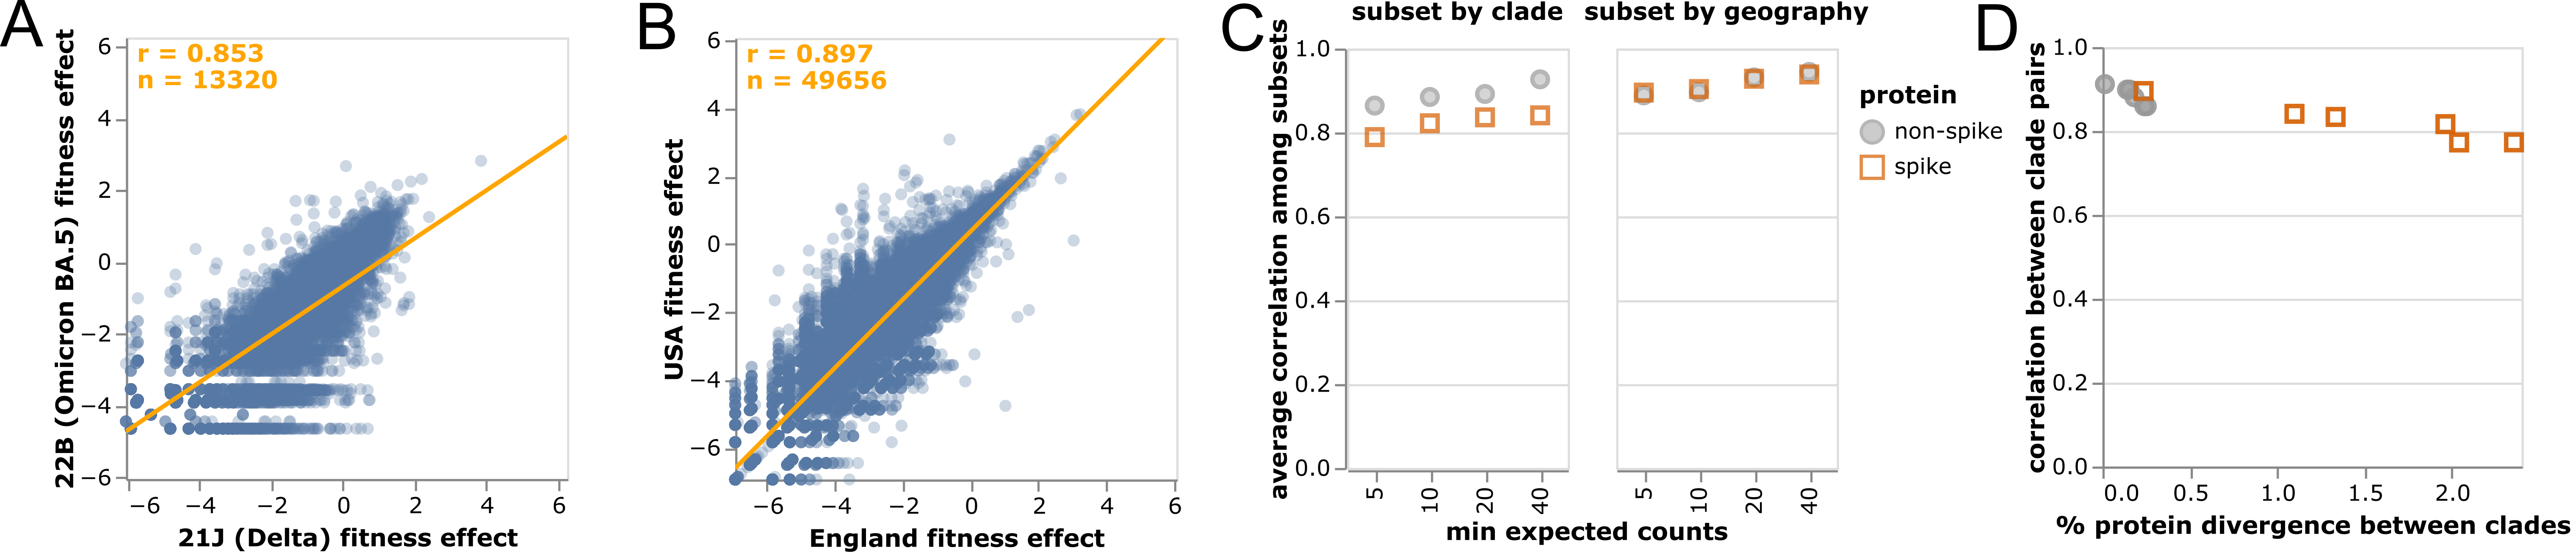
\includegraphics[width=\linewidth]{figs/corr.png}
\caption{
Correlations of mutation fitness effect estimates made using subsets of natural sequences.
Correlations between estimates made {\bf (A)} just using sequences from the Delta or Omicron BA.5 clades or {\bf (B)} just from the USA or England.
Each point is an amino-acid mutation, and orange text at upper left shows the number of mutations and Pearson correlation coefficient.
Only mutations with at least 10 expected counts are shown, which is why panels have different numbers of mutations shown (sequence subsets vary in size).
{\bf (C)} Correlations between clade or geography subsets become higher with an increasingly large threshold for minimum expected counts.
Spike mutations have a worse correlation when subsetting by viral clade (plot shows average correlation over all pairwise combinations of Delta, BA.1, BA.2, and BA.5), but not when subsetting by geography (USA or England).
{\bf (D)} Correlations in estimated mutation effects decline for clades with higher protein divergence, with the effect most noticeable for spike since spike is more diverged among SARS-CoV-2 clades than other viral proteins.
See \url{https://jbloomlab.github.io/SARS2-mut-fitness/clade_corr_chart.html} and \url{https://jbloomlab.github.io/SARS2-mut-fitness/subset_corr_chart.html} for versions of A and B that include all viral clades with at least 500,000 total expected counts (summed across all mutations) and have other interactive options.
\label{fig:corr}
}
\end{figure*}

We computed the correlations among mutation-effect estimates made using subsets of SARS-CoV-2 sequences from different viral clades or geographic locations.
These estimates were highly correlated, although there is modest variation in estimates across sequence subsets (Figure~\ref{fig:corr}A,B).

The modest variation in estimates from different sequence subsets could have two causes: statistical noise due to finite mutation counts, or real differences in effects of mutations among subsets of SARS-CoV-2.
It is not obvious why there should be real differences in mutation effects by geographic location, but there is experimental evidence that epistasis has shifted effects of some spike mutations during viral evolution~\citep{starr2022shifting,moulana2022compensatory,mccallum2021n}.
To test for statistical noise, we computed correlations with different thresholds for how many expected counts are required before making an estimate for a mutation (Figure~\ref{fig:corr}C).
Correlations increased with this count threshold, consistent with a reduction in statistical noise with larger mutation counts.
But the correlation for spike mutations was consistently lower for cross-clade but not cross-geography comparisons (Figure~\ref{fig:corr}C).
The lower cross-clade correlation for spike appears to be due to epistatic shifts in mutation effects that arise as sequences diverge~\citep{starr2022shifting, pollock2012amino, shah2015contingency}, since the correlation is lower between clades with higher spike divergence (Figure~\ref{fig:corr}D).
However, for the rest of this paper we aggregate counts across clades, since for most purposes the benefits aggregating counts (which enables lower-noise estimates for more mutations) outweighs the effect of modest epistatic shifts.

\subsection*{Structural and non-structural proteins are under strong purifying selection, but most accessory proteins are not}

\begin{figure*}
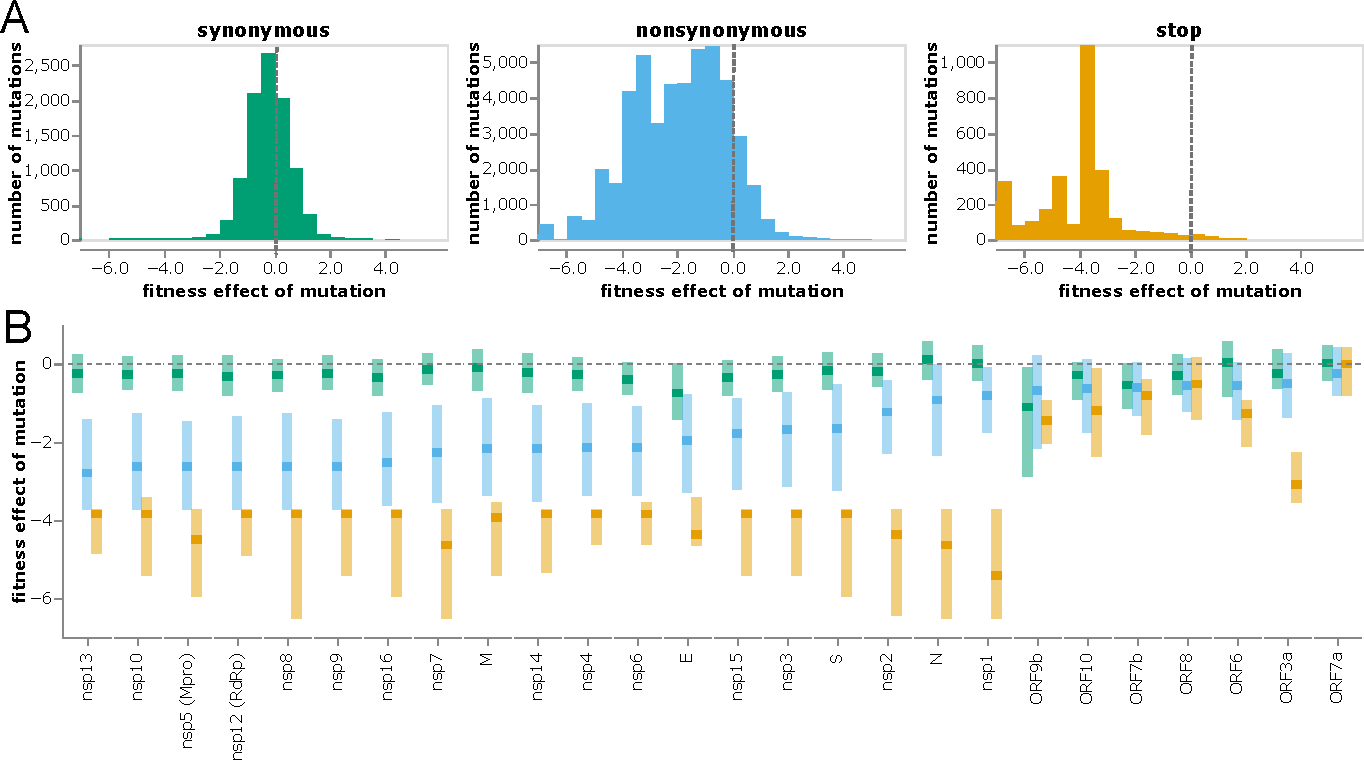
\includegraphics[width=\linewidth]{figs/dist.pdf}
\caption{
Distribution of effects of different classes of mutations.
{\bf (A)}
Histograms of effects of synonymous, nonsynonymous, and stop-codon mutations across all viral genes.
Neutral mutations have effects of zero (dashed gray vertical lines), and deleterious mutations have negative effects.
{\bf (B)}
Effects of each class of mutation for each viral gene.
Dark squares indicate the median effect, and the lighter rectangles span the interquartile range.
Mutation types are color-coded as in panel A.
See \url{https://jbloomlab.github.io/SARS2-mut-fitness/effects_histogram.html} and \url{https://jbloomlab.github.io/SARS2-mut-fitness/effects_dist.html} for plots that allow adjustment of the expected-count cutoff and other interactive options (such as separate histograms for each gene).
\label{fig:dist}
}
\end{figure*}

The distributions of mutation effects concur with biological intuition about how different classes of mutations impact protein function.
Most synonymous mutations are nearly neutral, most stop codons are highly deleterious, and amino-acid mutations range from slightly beneficial to highly deleterious (Figure~\ref{fig:dist}A).

To investigate differences among viral proteins, we computed the distributions of effects separately for each gene (Figure~\ref{fig:dist}B).
SARS-CoV-2 proteins are grouped into three categories: nonstructural (or nsp) proteins, structural proteins (spike, M, N, and E), and accessory proteins (names prefixed with ``ORF'')~\citep{v2021coronavirus}.
The nonstructural and structural proteins are essential, and these proteins show strong selection against stop codons and clear although variable purifying selection against amino-acid mutations (Figure~\ref{fig:dist}B; e.g., nsp13 is under stronger protein-level constraint than nsp1).

However, most accessory proteins are under little constraint (Figure~\ref{fig:dist}B).
Stop-codon and amino-acid mutations to ORF7a and ORF8 are not more deleterious than synonymous mutations.
The lack of deleterious mutations to ORF8 is consistent with the fact that viruses with deletions in this gene have spread in humans~\citep{su2020discovery}.
The only accessory protein under strong purifying selection against stop codons is ORF3a (Figure~\ref{fig:dist}B), for which stop codons in the first ~240 residues are clearly deleterious (Figure~\ref{fig:ORF3a}).
These observations concur with experiments showing SARS-CoV-2 is attenuated by deletion of ORF3a but there is little effect of deleting ORF6, ORF7a, or ORF8~\citep{mcgrath2022sars,silvas2021contribution,liu2022live}.
However, ORF3a's function must be relatively insensitive to its protein sequence, since other than selection against stop codons there is only amino-acid level constraint at a few sites like 135 and 138 (Figure~\ref{fig:ORF3a}).
Observations such as these could help guide experimental studies to better understand protein function.

\subsection*{Mutation-effect estimates correlate well with deep mutational scanning}

\begin{figure*}
\centering
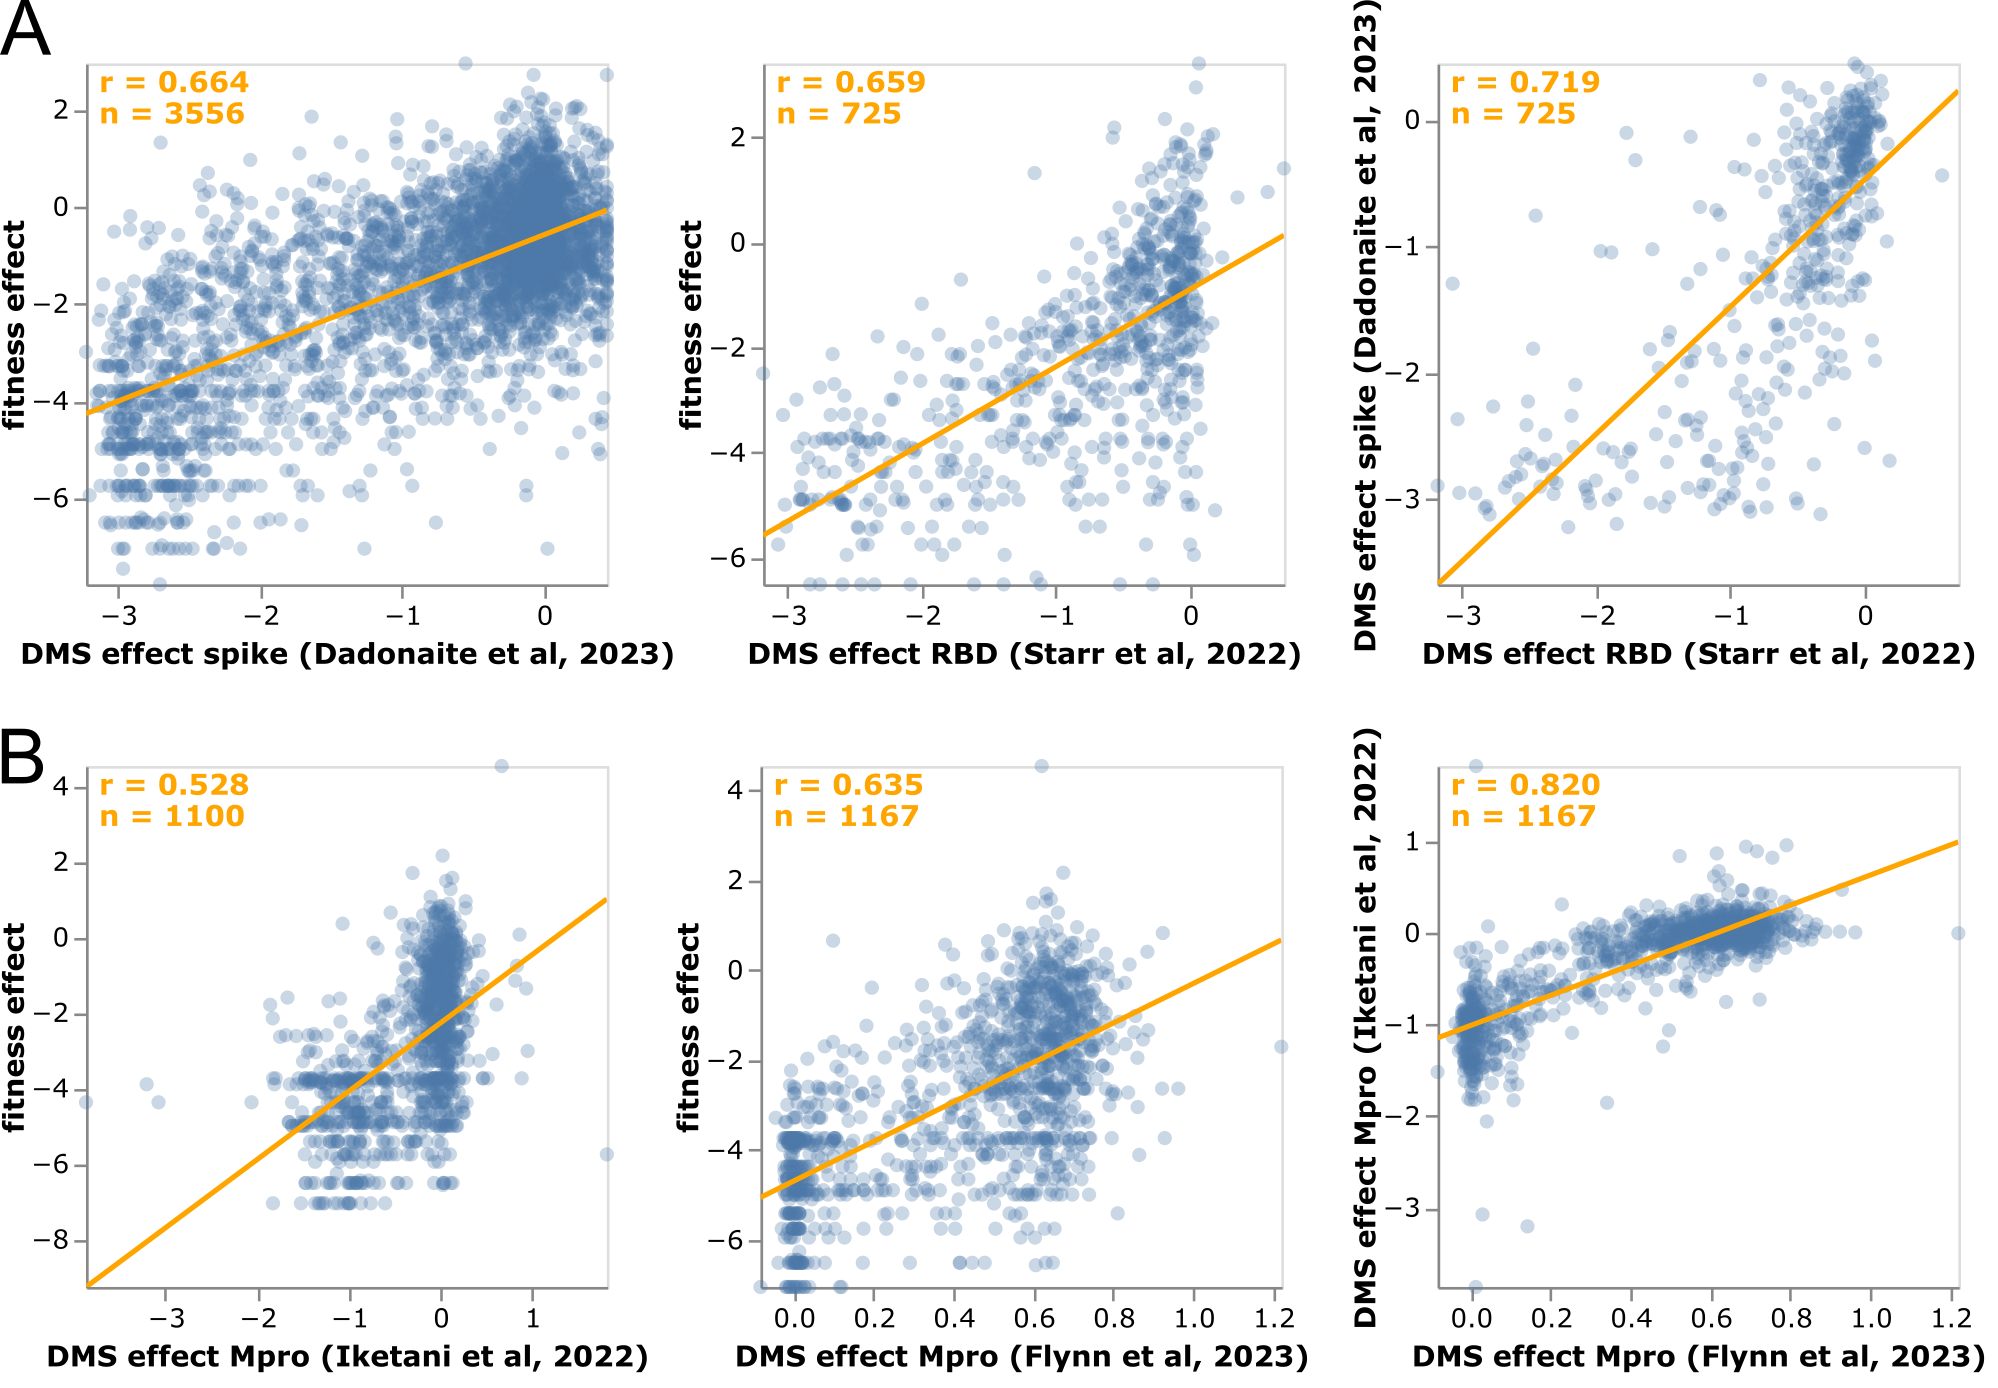
\includegraphics[width=0.75\linewidth]{figs/dms.png}
\caption{
Correlation of amino-acid fitness estimates with experimental measurements from deep mutational scanning studies for {\bf (A)} spike and {\bf (B)} Mpro (nsp5).
Each point is an amino-acid mutation, and the orange text in the upper left shows the number of mutations and Pearson correlation coefficient.
Data are taken from two independent deep mutational scanning studies for spike~\citep{cite}, and two studies for Mpro~\citep{cite}.
Each sub-panel shows a different set of mutations (depending on which mutations were measured in that experiment).
See \url{https://jbloomlab.github.io/SARS2-mut-fitness/dms_S_corr.html} and \url{https://jbloomlab.github.io/SARS2-mut-fitness/dms_nsp5_corr.html} for interactive versions of these plots that enable subsetting on just mutations shared across all datasets, and adjustment of the minimum expected count cutoff .
\label{fig:dms_corr}
}
\end{figure*}

\subsection*{Interactive exploration of amino-acid fitnesses}

\begin{figure*}
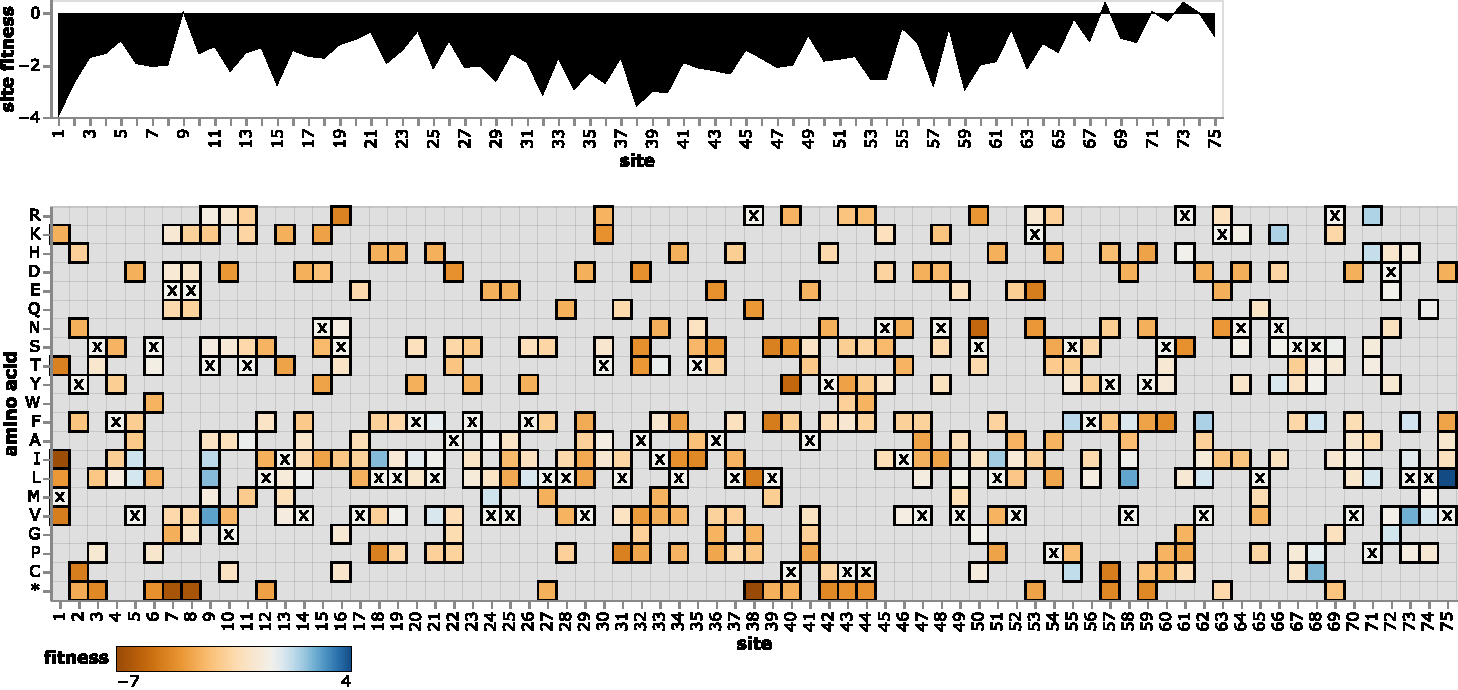
\includegraphics[width=\linewidth]{figs/E_heatmap.pdf}
\caption{
Effects of amino-acid mutations to E protein.
The area plot at top shows the average effects of mutations at each site, and the heatmap shows the effects of specific amino acids, with \textbf{x} denoting the amino-acid identity in the Wuhan-Hu-1 strain.
Only mutations with at least 10 expected counts are shown.
See \url{https://jbloomlab.github.io/SARS2-mut-fitness/E.html} for an interactive version of this plot that enables zooming, mouseovers, and adjustment of the minimum expected count threshold.
See the links at \url{https://jbloomlab.github.io/SARS2-mut-fitness} for comparable interactive plots for all other SARS-CoV-2 proteins.
\label{fig:E_heatmap}
}
\end{figure*}

\begin{figure*}
\centering
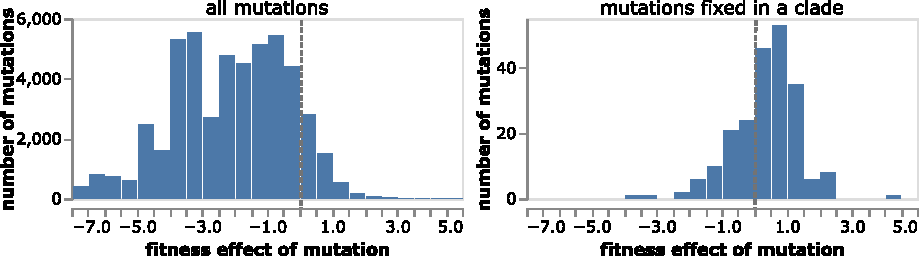
\includegraphics[width=0.7\linewidth]{figs/fixed_dist.pdf}
\caption{
Distribution of fitness effects of all amino-acid mutations relative to Wuhan-Hu-1, and all mutations that fixed in at least one clade of SARS-CoV-2 (using the Nextstrain clade definitions).
The vertical dashed line at zero indicates the effect of a neutral mutation.
Estimates are only shown for mutations with expected counts of at least 10.
See \url{https://jbloomlab.github.io/SARS2-mut-fitness/clade_fixed_muts_hist.html} for an interactive version of this plot that allows adjustment of the minimum expected count threshold.
\label{fig:fixed_dist}
}
\end{figure*}

\section{Discussion}

Caveats include synonymous selection.

{\small

\section{Methods}
\subsection{Code and data availability}
Code and data are at \url{https://github.com/jbloomlab/SARS2-mut-fitness}.

\section{Acknowledgments}
We thank Angie Hinrichs for assistance with resolving several questions related to use of the UShER package and its pre-built mutation-annotated tree \jdbcomment{if we don't add as co-author}.
\jdbcomment{Jesse to acknowledge AVIDD, CEIRR, and R01 grants.}
JDB is an Investigator of the Howard Hughes Medical Institute.

\section{Competing interests}
JDB is on the scientific advisory boards of Apriori Bio, Aerium Therapeutics, Invivyd, the Vaccine Company, and Oncorus.
JDB receives payments as an inventor on a Fred Hutch licensed patents related to deep mutational scanning of viral proteins.

\bibliography{references}
}

\onecolumn
\renewcommand{\thepage}{S\arabic{page}}
\setcounter{page}{1}
\renewcommand{\thefigure}{S\arabic{figure}}
\setcounter{figure}{0}

\clearpage

\section{Supplementary Material}

\begin{figure*}[h]
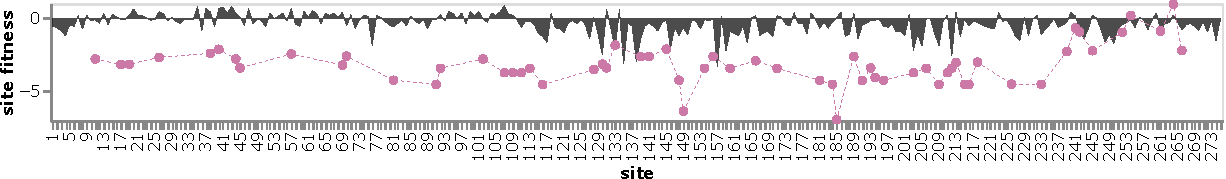
\includegraphics[width=\linewidth]{figs/ORF3a.pdf}
\caption{
Effects of stop-codon and amino-acid mutations across ORF3a.
The black area plot shows the mean effect of all amino-acid mutations at each site, and the purple points show the effects of stop codon mutations.
There is strong selection against stop codons (negative effects) for all but the C-terminus of ORF3a, but only a few positions show strong selection against amino-acid substitutions.
This plot shows only mutations with 20 expected counts.
See \url{https://jbloomlab.github.io/SARS2-mut-fitness/ORF3a.html} for an interactive version of this plot along with zoomable heatmap of the effects of specific amino-acid substitutions.
\label{fig:ORF3a}
}
\end{figure*}

\begin{figure*}[b]
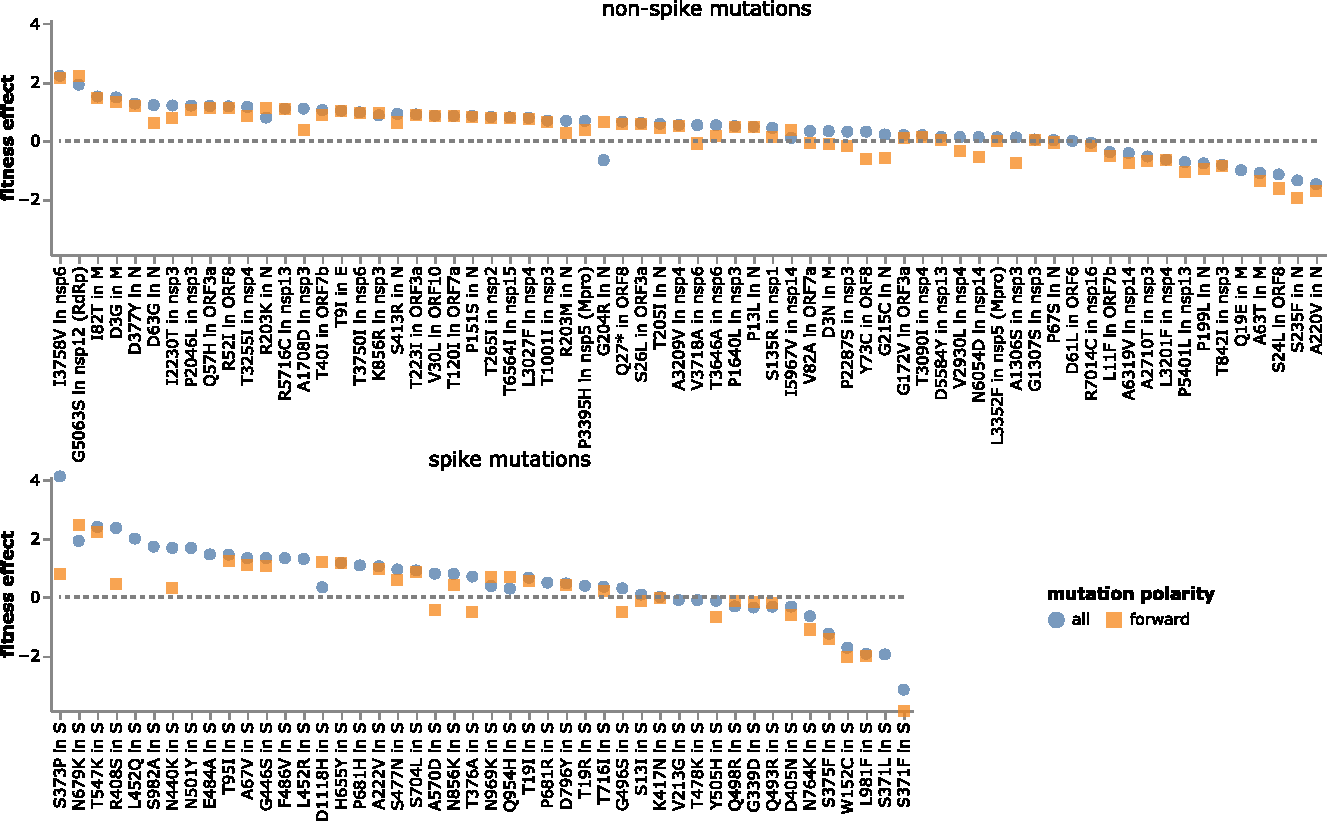
\includegraphics[width=\linewidth]{figs/fixed.pdf}
\caption{
Effects of individual mutations that fixed in at least one clade of SARS-CoV-2, faceted by whether they are in spike or another protein.
Plots show estimates of effects of mutations made across all clades (including those that have fixed the mutation) and just from direct forward occurrences of the mutation in clades in which it has not yet fixed.
Estimates are only shown for mutations with expected counts of at least 10.
See \url{https://jbloomlab.github.io/SARS2-mut-fitness/clade_fixed_muts.html} for an interactive version of this plot.
\label{fig:fixed}
}
\end{figure*}


\begin{figure*}
\centering
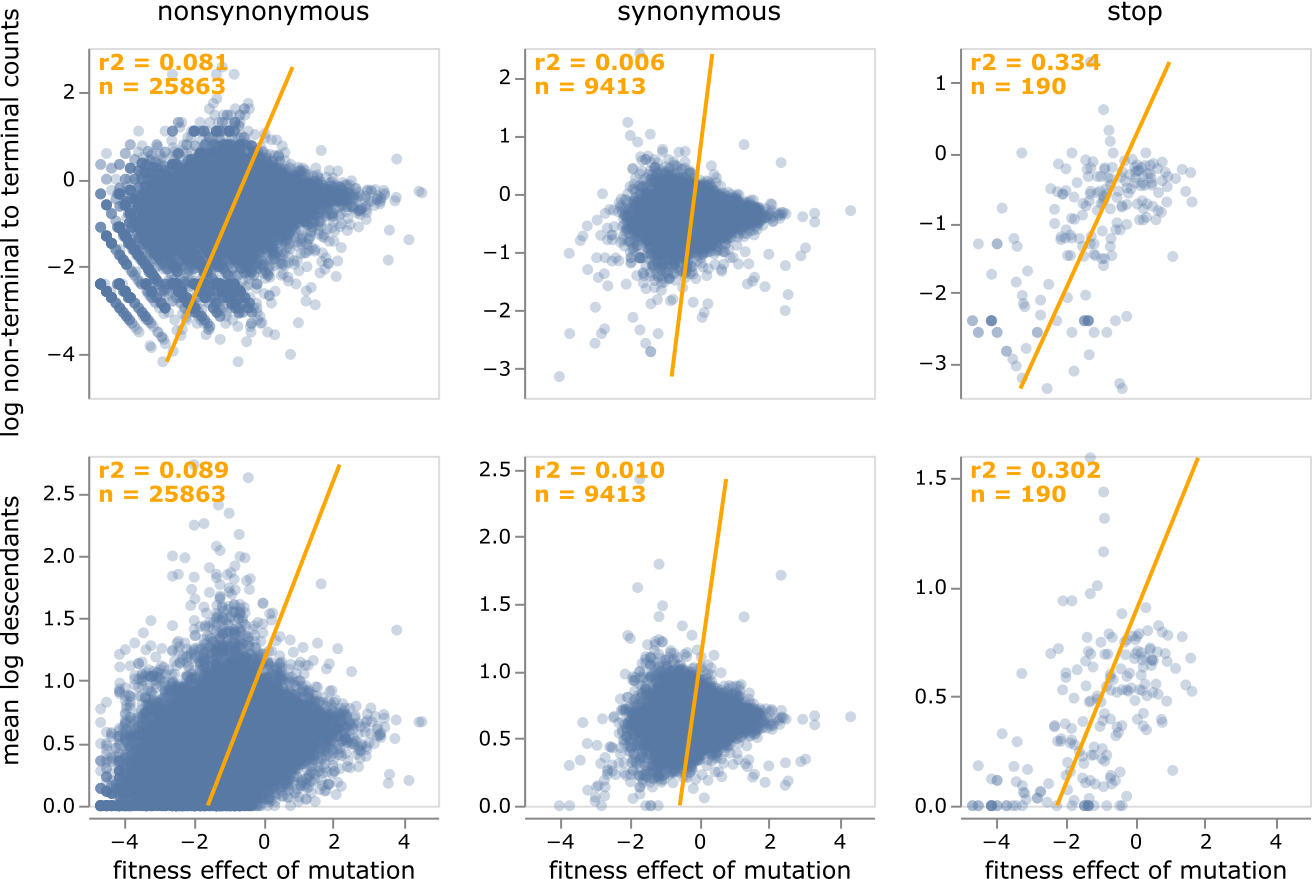
\includegraphics[width=0.75\linewidth]{figs/terminal.png}
\caption{
Relationship between fitness effects of mutations and ratio of counts on terminal (tip) branches versus non-terminal (internal) branches.
Each point is an amino-acid mutation, and the orange text in the upper left give the number of mutations and the Pearson correlation coefficient.
This plot shows only mutations with at least 10 expected counts and 5 actual counts.
See \url{https://jbloomlab.github.io/SARS2-mut-fitness/fitness_vs_terminal.html} for an interactive version of this plot that allows filtering by the number of actual or expected counts, or by gene.
\label{fig:terminal}
}
\end{figure*}

\end{document}
